\documentclass[12pt,a4paper]{article}
\usepackage[utf8]{inputenc}
\usepackage[german]{babel}
\usepackage[T1]{fontenc}
\usepackage{amsmath}
\usepackage{amsfonts}
\usepackage{amssymb}
\usepackage{graphicx}
\usepackage{float}
\usepackage[left=2cm,right=2cm,top=2cm,bottom=2cm]{geometry}
\author{Tim}

\begin{document}

\tableofcontents
\newpage

\section{Kondensator}
\subsection{Versuchsbeschreibung}
In diesem Teilversuch soll die Kapazität eines Kondensators durch Auf- und Entladung von diesem bestimmt werden.
\subsubsection{Aufladung}
Wird eine Spannung an einen Kondensator angelegt, so wird dieser geladen, bis die Quellspannung kompensiert wird. Der Ladevorgang dauert umso länger, je größer der Widerstand des Stromkreises ist.\\
Aus der Maschenregel folgt:
\begin{equation}
U_0 = U_R + U_C \Rightarrow U_0 - U_C = R\cdot C\cdot \dfrac{dU_c}{dt}
\label{Kondensator_DGL}
\end{equation}
Bei der Aufladung kann man daraus den Strom und die Spannung bestimmen:
\begin{equation}
U_C(t) = U_0 \cdot (1-e^{-\dfrac{t}{R\cdot C}})
\end{equation}
\begin{equation}
I(t) = I_0 \cdot e^{-\dfrac{t}{R\cdot C}}
\end{equation}
Dabei ist $\tau = R \cdot C$ die Zeitkonstante des R-C-Kreises.
\subsubsection{Entladung}
Bei der Entladung liegt keine externe Spannung mehr an. Es gilt also: $U_0 = 0$\\
Mit dieser Annahme und Gl. \ref{Kondensator_DGL} folgt:
\begin{equation}
U_C(t) = U_0 \cdot e^{-\dfrac{t}{R\cdot C}}
\end{equation}
\begin{equation}
I(t) = -I_0 \cdot e^{-\dfrac{t}{R\cdot C}}
\end{equation}
\subsection{Aufbau und Durchführung}
\begin{figure}[H]
\begin{center}
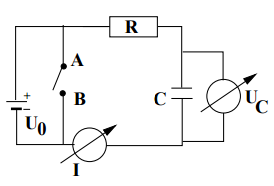
\includegraphics[width=0.75\linewidth]{Bilder/Kondensator_Aufbau}
\caption[Aufbau Kondensator]{Aufbau Kondensator}
\label{fig:Kond_Aufbau}
\end{center}
\end{figure}

\begin{tabular}{|c|c|c|}
\hline 
Bauteil & Angegebener Wert & Bestimmter Wert \\ 
\hline 
Widerstand & 100 & • \\ 
\hline 
Kondensator & 4.7 & 4.88 \\ 
\hline 
\end{tabular} 

Der Versuch wird gemäß Abb. \ref{fig:Kond_Aufbau} aufgebaut. Dabei wird als Spannungsquelle die des CASSY benutzt.Diese wird mit dem Stromkreis, bestehend aus einem Widerstand, einem Kondensator und dem Strommessgerät, verbunden. Um die Entladung des Kondensators durchführen zu können wird noch ein Schalter so eingebaut, dass die Spannungsquelle kurzgeschlossen werden kann.\\ 
Die Bauteileigenschaften  der verwendeten Teile sind in Tabelle ... aufgelistet.
Über Kanal A des CASSY wird der Stromfluss gemessen und über Kanal B die Spannung am Kondensator.\\
Gleichzeitig wird auch Strom und Spannung mit einem Oszilloskop gemessen. Dafür wird an Kanal 2 des Oszilloskopes der Spannungsabfall über den Widerstand und an Kanal 1 die Spannung über den Kondensator angeschlossen. Die Erde wird zwischen Kondensator und Widerstand gelegt.\\
\\
Um den Aufladevorgang zu messen, wird die Spannungsquelle beim Start einer Messung aktiviert.
Beim Entladevorgang bleibt die Spannungsquelle eingeschaltet. Der Messvorgang wird über einen Trigger gestartet, der den Spannungsabfall registriert.
\subsubsection{Messung mit dem Oszilloskop}
\begin{tabular}{c c c}
\hline 
Messparameter & Zeitauflösung: $500\mu s$  & Spannungsauflösung: $0.2V$ \\ 
\hline
\end{tabular} 
\subsubsection{Messung mit CASSY}
\begin{tabular}{c c c c}
Messparameter & Messintervall: $10\mu s$  & Anzahl Messwerte: 1000 & automatische Aufnahme \\ 
Messbereiche & Strom: 0.3A & Spannung: 3V \\
Trigger: 2V & angelegte Spannung: 2.1V\\
\end{tabular} 

\subsection{Auswertung Oszilloskop}
Während der Versuchdurchführung wurde bereits mit dem Oszilloskop eine Schnellauswertung durchgeführt.
Um die Kapazität zu bestimmen wurden jeweils bei Auf- und Entladung zwei Zeiten mit dazugehörigen Spannungen aufgenommen. Dabei wurden immer Werte an der Spannungskurve aufgenommen, da die Stromkurve sehr starke Schwankungen hatte und dadurch vermutlich ungenauer gewesen wäre. Die gemessenen Werte sind in Tab... aufgeführt. Die Kapazität wird folgendermaßen bestimmt:
\begin{equation}
\dfrac{U1}{U2} = e^{-\dfrac{t1-t2}{R\cdot C}}
\end{equation}
Nach C auflösen ergibt:
\begin{equation}
C = \dfrac{t1-t2}{R\cdot \ln(\dfrac{U1}{U2}}
\end{equation}


\begin{tabular}{|c|c|c|c|c|c|}
\hline 
• & Offset & t1 & U1 & t2 & U2 \\ 
\hline 
Aufladung & -1.18V & -5.2ms & -0.928V & $0.5ms$ & -0.240V \\ 
\hline 
Entladung & -16mV & $0.34ms$ & -1.18V & $0.98ms$ & -0.08V \\ 
\hline 
\end{tabular} 
Die statistischen Fehler dieser Werte ist durch die Ableseungenauigkeit bestimmt. Dabei gilt:
\begin{equation}
\sigma_t = \dfrac{0.1ms}{\sqrt{12}} = 0.03ms
\end{equation}
\begin{equation}
\sigma_U = \dfrac{0.01V}{\sqrt{12}} = 0.003V
\end{equation}

\begin{tabular}{|c|c|}
\hline 
• & Gemessener Wert \\ 
\hline 
Aufladung & $4.69\pm 0.05\pm 0.08$ \\ 
\hline 
Entladung & $4.88\pm 0.02\pm 0.05$ \\ 
\hline 
\end{tabular} 
\begin{equation}
\sigma_{C_stat} = \sqrt{2\cdot\left(\dfrac{\sigma_t}{R\cdot ln(\dfrac{U1}{U2})}\right)^{2}+\left(\dfrac{-\sigma_U\cdot(t1-t2)}{R\cdot U1\cdot ln(\dfrac{U1}{U2})^{2}}\right)^{2}+\left(\dfrac{\sigma_U\cdot(t1-t2)}{R\cdot U2\cdot ln(\dfrac{U1}{U2})^{2}}\right)^{2}}
\end{equation}
\begin{equation}
\sigma_{C_sys} = \dfrac{(t2-t1)\cdot \sigma_R}{R^{2}\cdot ln(\dfrac{U1}{U2}}
\end{equation}

\subsection{Auswertung CASSY}
Es wurden ebenfalls Werte über das CASSY aufgezeichnet.
\subsubsection{Rohdaten}
\begin{figure}[H]
\begin{center}
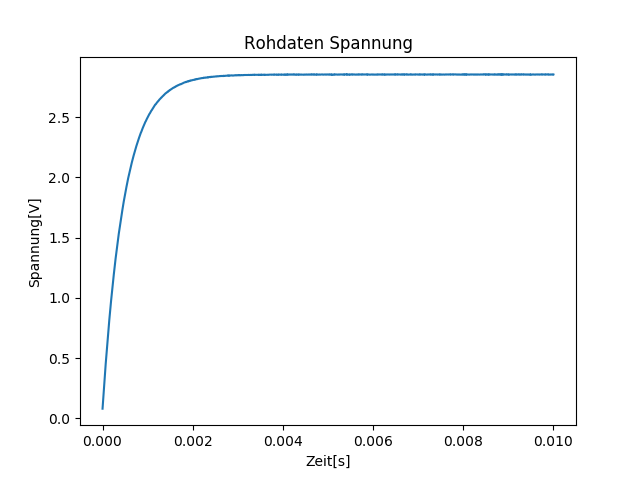
\includegraphics[width=0.75\linewidth]{Bilder/Kondensator_U}
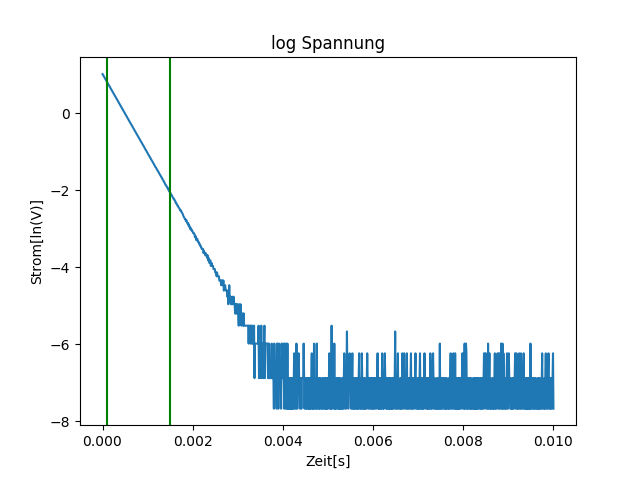
\includegraphics[width=0.75\linewidth]{Bilder/Kondensator_logU}
\caption[Rohdaten logarith. A]{Rohdaten Spannung}
\label{fig:RohU}
\end{center}
\end{figure}

\begin{figure}[H]
\begin{center}
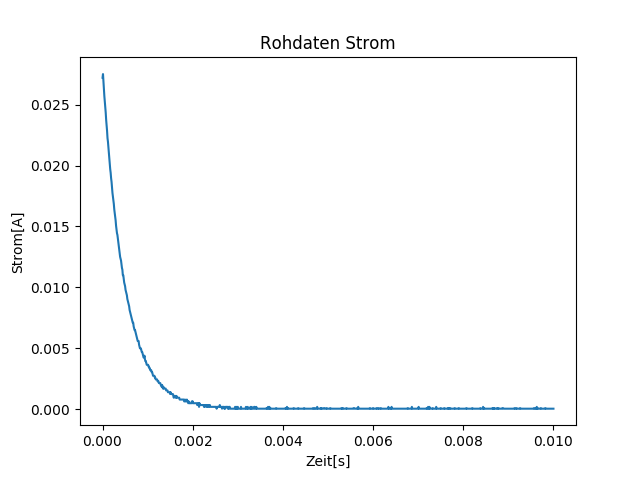
\includegraphics[width=0.75\linewidth]{Bilder/Kondensator_I}
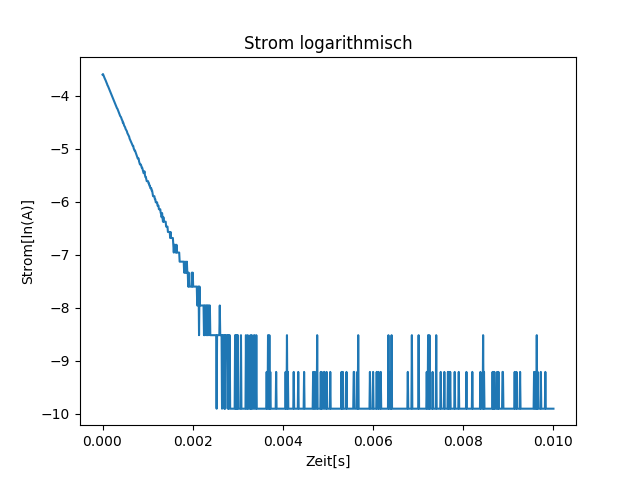
\includegraphics[width=0.75\linewidth]{Bilder/Kondensator_logI}
\caption[Rohdaten logarith. A]{Rohdaten Spannung}
\label{fig:RohU}
\end{center}
\end{figure}

\subsubsection{lineare Regressionen}

\section{RLC-Schwingkreis}
\subsection{Versuchsbeschreibung}

In diesem Versuch soll die gedämpfte Schwingung eines RLC-Schwingkreises aufgezeichnet werden, sowie die Schwingungsfrequenz und Dämpfung der Schwingung bestimmt werden.
Mit diesen Werten sollen gegebenenfalls die verwendeten Bauteile charakterisiert werden.

\subsubsection{Grundlagen}
Grundlage des Versuchs ist die gedämpfte Schwingungsgleichung bei der Entladung des Kondensators

\begin{equation}
\ddot{Q}+2\delta \dot{Q}+\omega_0^2 Q=0
\end{equation}

mit der Dämpfung $\delta=\frac{R}{2L}$ und der Kreisfrequenz der ungedämpften Schwingung $\omega_0=\frac{1}{\sqrt{LC}}$.\\
Dabei müssen drei Fälle unterschieden werden:\\
Im \textbf{Kriechfall} gilt $\delta > \omega_0$. Die Spannung fällt asymptotisch gegen null ab und es findet keine Schwingung statt.\\
Der \textbf{Aperiodischer Grenzfall} liegt vor falls $\delta=\omega_0$. Der Kondensator wird in kürzester Zeit und ohne Überschwingen entladen.\\
Für $\delta<\omega_0$ liegt der \textbf{Schwingfall} vor. Die Spannungssignal ist von der Form 
\begin{equation}
U_c(t)=U_0 \cdot e^{-\delta t} \cdot \sin{\omega t} \quad \text{mit} \quad \omega=\sqrt{\omega_0^2-\delta^2}
\end{equation}
und erreicht erst nach einem Einschwingvorgang seinen Endwert.\\

Eine Charakterisierung der verwendeten Spule wird dabei über folgende Zusammenhänge ermöglicht:
\begin{equation}
L=\frac{1}{(\omega^2+\delta^2)\cdot C} \qquad  R_L=\frac{2\delta}{(\omega^2+\delta^2)\cdot C}-R_{gesteckt}
\end{equation}

\subsection{Aufbau und Durchführung}
\subsubsection{Aufbau}

Der Schwingkreis wird gemäß dem Schaltplan (Abb. \ref{fig:RLCSchaltung}) aufgebaut. Als Widerstand wurde ein Potentiometer verwendet. Der hier verwendete Kondensator hatte eine nominelle Kapazität von $C=4.7 \mu F$, für die verwendete Spule waren $R_L=9.5 \Omega$ und $L \approx 36mH$ ausgewiesen. Strom und Spannung werden mit dem CASSY gemessen. Die Einstellungen finden sich in Tab. \ref{tab:CASSY}

\begin{figure}
\begin{center}
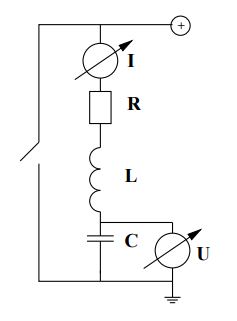
\includegraphics[scale=0.8]{Bilder/RLCSchaltung.png}
\end{center}
\caption[RLC Schaltung]{Schaltplan des RLC-Schwingkreises. (Quelle: Praktikumsskript Seite 84)}
\label{fig:RLCSchaltung}
\end{figure}

\begin{table}
\begin{center}
\begin{tabular}{|c|c|}
\hline
Messparameter &  $10 \mu s$ Messintervall;  2000 Messwerte \\
\hline
Einstellungen & Messbereich U: -10V bis 10V\\
\hline
Trigger & fallend, 6V\\
\hline
Anm. & \\
\hline
\end{tabular}
\caption[CASSY]{Einstellungen CASSY}
\label{tab:CASSY}
\end{center}
\end{table}


\subsubsection{Durchführung}
Es wird die durch Entladen des Kondensators angeregte Schwingung aufgezeichnet. Dazu wird der Kondensator zunächst mit 7V Ladespannung geladen. Nach Einstellen des Widerstandes am Potentiometer (Eingesteller Wert wurde mit dem Multimeter bestimmt) wird der Schalter geschlossen. Durch den Kurzschluss der Spannungsquelle entlädt sich der Kondensator über den Widerstand. Der Verlauf der Kondensatorspannung und des Stroms werden aufgezeichnet.\\
Der Entladevorgang wurde für jede Widerstandseinstellung insgesamt fünf mal durchgeführt.


\subsection{Auswertung}
\subsubsection{Rohdaten}
Der prinzipielle Verlauf ist bei fast allen Messungen weitesgehend identisch, deswegen werden hier nur einige Spannungsverläufe exemplarisch gezeigt.

\begin{figure}
\begin{center}
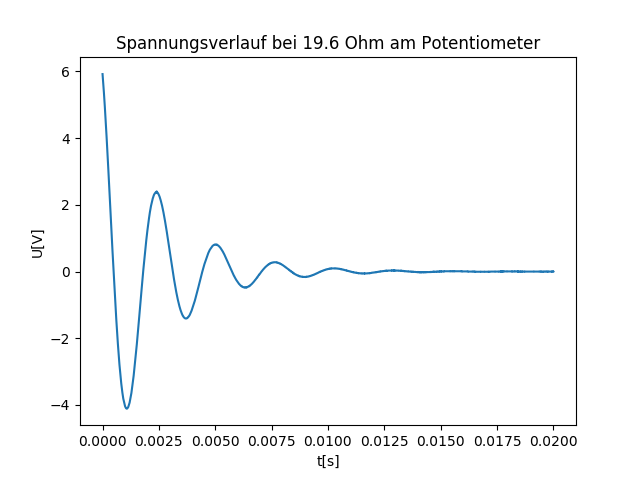
\includegraphics[scale=0.75]{Bilder/Spannungsverlauf19,6Ohm}
\end{center}
\caption[Spannungsverlauf]{Spannungsverlauf für Messung 1 bei $R=19.6 \Omega$ am Potentiometer (Multimeterangabe).}
\label{fig:Spannung19,6}
\end{figure}

...to be continued....

\subsubsection{Frequenzbestimmung}
In diesem Versuch stehen einem prinzipiell zwei Möglichkeiten zur Frequenzbestimmung zur Verfügung.
Einmal durch Fouriertransformation des gemessenen Spannungssignals und anschließender Peakbestimmung, die zweite Möglichkeit durch Bestimmung der mittleren Periodendauer des Spannungssignals.\\

Die Bestimmung mittels Fouriertransformation ist in diesem Fall nicht zufriedenstellend, da die Auflösung des Spektrums zu grob ist (siehe Abb.\ref{fig:Fourier19,6} für das zu Abb.\ref{fig:Spannung19,6} zugehörige Frequenzspektrum).\\

\begin{figure}
\begin{center}
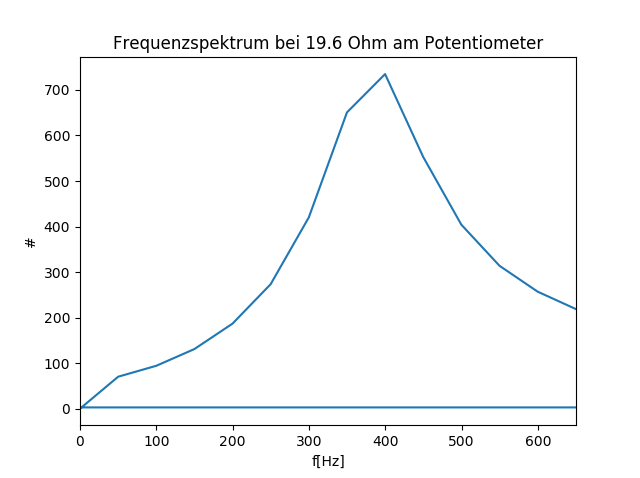
\includegraphics[scale=0.75]{Bilder/fft_19,6Ohm}
\end{center}
\caption{Frequenzspektrum von Messung 1 bei $R=19.6 \Omega$. Die Auflösung ist mit $\approx 50Hz$ viel zu grob.}
\label{fig:Fourier19,6}
\end{figure}

Für die Bestimmung der Frequenz aus der mittleren Periodendauer sind bessere Ergebnisse erzielt worden.\\
Dazu wurden im Spannungssignal Vorzeichenwechsel gesucht. Die Nullstelle ist dann der Mittelwert der Zeitpunkte eines solchen Vorzeichenwechsels, als Fehler auf die Nullstelle wurde eine Gleichverteilung zwischen den beiden Zeitpunkten angenommen. Es ergibt sich dann für Nullstellen $t_i$:

\begin{equation}
t_i=(t_++t_-)/2 \quad \quad \quad
\sigma_{t_i}=\frac{t_+-t_-}{\sqrt{12}}
\end{equation}

Mit der Zeitspanne zwischen zwei Nullstellen ergibt sich für die Periodendauer:

\begin{equation}
T_i=2\cdot (t_{i+1}-t_i) \quad \quad
\sigma_{T_i}=2\cdot \sqrt{\sigma_{t_{i+1}}^2+\sigma_{t_i}^2}
\end{equation}

Mittels Mittelwert und Fehler auf diesen ergibt sich für jede der fünf Messungen pro eingestelltem Widerstand eine mittlere Periodendauer mit Fehler. Mittels einem gewichteten Mittelwert werden diese zu einem Endergebnis für jede Widerstandseinstellung zusammengefasst.\\
Für die Frequenz folgt dann:

\begin{equation}
f=\frac{1}{\overline{T}} \quad \quad \quad
\sigma_f=\frac{\sigma_{\overline{T}}}{\overline{T}^2}
\end{equation}

Eine Zusammenstellung der auf diese Weise gewonnen Frequenzen bei diversen Widerstandseinstellungen finden sich in Tabelle \ref{tab:Frequenzen}.

\begin{table}
\begin{center}
\begin{tabular}{|c|c|c|}
\hline
$R[\Omega]$ & $f[Hz]$ & $\sigma_f[Hz]$ \\
\hline
 19.6 & 382.78 & 0.16\\
\hline
 28.5 & 376.84 & 0.18\\
\hline
 38.9 & 373.21 & 0.20\\
\hline
 52.2 & 364.84 & 0.22\\
\hline
 68.8 & 350.75 & 0.24\\
\hline
\end{tabular}
\end{center}
\caption{Ergebnisse der Frequenzbestimmung durch Nullstellen}
\label{tab:Frequenzen}
\end{table}



\subsubsection{Charakterisierung des Kondensators}
Mit den zuvor ermittelten Werten für die Dämpfung, die Schwingungsfrequenz und die Induktivität kann der verwendete Kondensator charakterisiert werden. Man nutzt dafür den Zusammenhang:

\begin{equation}
C_i=\frac{1}{(\omega_i^2+\delta_i^2)\cdot L} \quad \quad 
\sigma_{C_i}=\frac{\sqrt{\sigma_L(\omega_i^2+\delta_i^2)+2\omega_i L \sigma_{\omega_i}+2 \delta_i L \sigma_{\delta_i}}}{(\omega_i^2+\delta_i^2)L} 
\end{equation}

Die Einzelergebnisse werden dann durch den gewichteten Mittelwert zusammengefasst.



\subsubsection{Aperiodischer Grenzfall}



\section{Gekoppelte Schwingkreise}
\subsection{Versuchsbeschreibung}
Ein LC-Schwingkreis kann induktiv mit einem zweiten LC-Schwingkreis gekoppelt werden, der dadurch zu erzwungenen Schwingungen angeregt wird. Falls die Eigenfrequenzen der Schwingkreise gleich ist $w_1 = w_2$, tritt eine Resonanz auf. In diesem Fall kann eine Schwebung beobachtet werden. Bedeutet: Die Schwingungsenergie "schwingt" zwischen den Schwingkreisen hin und her. \\
Bei diesem Versuch werden die Fundamentalschwingungen und die Schwebung zweier gekoppelter Schwingkreise aufgenommen. Die Differentialgleichungen der gekoppelten Schwingkreise lauten:
\begin{equation}
\ddot{I_1} + k \cdot \ddot{I_2} + \dfrac{I_1}{L \cdot C} = 0
\end{equation}
\begin{equation}
\ddot{I_2} + k \cdot \ddot{I_1} + \dfrac{I_2}{L \cdot C} = 0
\end{equation}
mit Kopplung k ($0 < k < 1)$ folgen die Eigenfrequenzen zu
\begin{equation}
\dfrac{w_0}{\sqrt{1+k}} = w_+ < w_0 < w_- = \dfrac{w_0}{\sqrt{1-k}} 
\end{equation}
Dabei ist $w_0$ die Eigenfrequenz des Schwingkreises im ungekoppelten Fall ($w_0 = \dfrac{1}{\sqrt{LC}}$)
Die Kopplung kann aus den Frequenzen der Fundamentalschwingungen berechnet werden:
\begin{equation}
k = \dfrac{f_-^2 - f_+^2}{f_-^2 + f_+^2}
\end{equation}
\\ Die Erwartung bei dieser Versuchskonfiguration ist, dass die Amplitudennullstellen des einen Schwingkreises mit einem Amplitudenextremum des anderen zusammenfallen. Die Dämpfung durch Ohm'sche Widerstände in allen Bauteilen verschiebt diese beiden allerdings gegeneinander. Für Kopplungen k < 0,2 lässt sich die Verschiebung näherungsweise berechnen:
\begin{equation}
\Delta t \approx \dfrac{1}{w_Schwebung} \cdot \left[\dfrac{\pi}{2} - \arctan \left( \dfrac{k}{R} \cdot \sqrt{\dfrac{L}{C}} \right)\right]
\end{equation}  
\subsection{Aufbau und Durchführung}
\subsection{Auswertung}










\end{document}